% !Mode:: "TeX:UTF-8"
%%% Local Variables:
%%% mode: latex
%%% TeX-master: t
%%% End:

% 绪论和个人工作

\chapter{绪论}
\label{cha:intro}
\section{引言}

近些年来,随着互联网的快速发展,人工智能和大数据技术的兴起和应用,网络知识、信息和数据大量增长,人们面对的数据越来越多。
传统的基于网页链接检索的信息存储、信息检索方式越来越难于进行查找学习知识,随着移动设备
的增加,人们对于信息检索、知识获取的要求也越来越高,面对各种数据信息,
人们查找检索知识的需求越来越迫切,越来越期望能更好更快的检索了解学习知识。
随之知识库构建、推理和应用变得流行起来,越来越多的大学、科研机构和商业公司开始构建大规模知识库,如Google Knowledge Graph\cite{Dong2014FromDF},NELL\cite{NELL-aaai15},YAGO\cite{Suchanek:2007:YCS:1242572.1242667},
Freebase\cite{Bollacker2008FreebaseAC},DBpedia\cite{Bizer:2009:DCP:1640541.1640848}等。
这些知识库基于自动和半自动的信息抽取、众包、专家领域内知识等方式进行构建,
把互联网、书籍、数据库等各处非结构化的文本中数据结构化、抽取构建知识库,
获得了大量的实体、关系和属性信息,能为人们提供的方便快捷的信息查询、检索、知识学习途径。
这类知识库的数据完整性、数据精确性和数据质量等衡量指标非常高,
已经有很多基于知识库的系统被成功用于商业领域,如谷歌搜索引擎\footnote{https://googleblog.blogspot.com/2012/05/introducing-knowledge-graph-things-not.html},
微软的必应搜索\footnote{https://blogs.bing.com/search/2013/03/21/understand-your-world-with-bing/}等。
除了这些通用领域的知识库之外,也有很多领域知识库被构建和应用,知识库也被用于生物学\cite{Dumontier:2014:BRL:2878453.2878554}、金融学、教育学等各个领域,一些较为成熟的问答系统、个人手机助手如苹果公司的Siri、谷歌公司的Google Assistant、微软公司的手机助手小冰、出门问问等也将知识库集成其中。

常见的知识库可以用有向图进行可视化表示,图\ref{kb}是一个简单的关于北京师范大学的知识库,描述了和北京师范大学相关的实体、属性和关系。图中展示了实体、实体和实体之间关系,其中实体是描述现实中实际存在的事物、地点、人物、事件如:北京师范大学、北京等,关系是描述实体和实体之间存在的某种联系和特征,如北京师范大学和北京存在着位于的关系。除此之外,
一个知识库中的三元组还可以分为关系型三元组和实体属性三元组。关系三元组典型的例子如:(北京师范大学,位于,北京)。其中“北京师范大学”和“北京”是实体,
属性事实三元组如:(北京,人口,2150万)。
其中“北京”是实体,“2150万”是描述实体属性的属性值,“人口”是北京这类实体具有的一种属性特征类型。通常实体关系三元组用来描述实体和实体之间的联系,实体属性三元组描述实体的属性事实特征,这些不同类型的三元组共同构成一个完整的知识库。

\begin{figure}[H]
\begin{center}
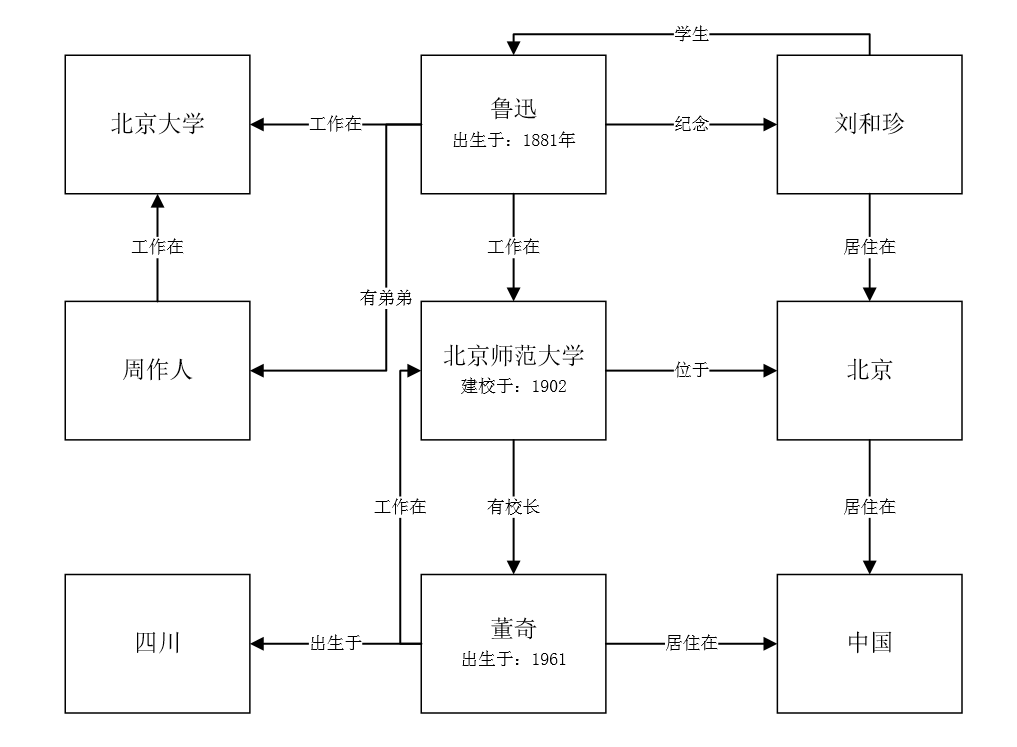
\includegraphics [width=0.8\textwidth]{kb2.PNG}
\caption{一个知识库例子}
\label{kb}
\end{center}
\end{figure}

\section{知识库补全问题}
本节介绍知识库补全算法的主要研究问题,了解知识库补全算法相关的难点。尽管一些知识库的三元组数量巨大,但这些知识库仍然是不完备的,如很多人的出生地点并未包含在知识库中,一些演员是否出演过某些电影也是未知的。为了能发掘知识库中隐藏的实体和实体之间的关系,有很多知识库补全算法被提出。

\subsection{关系路径特征和实体属性特征}
虽然许多知识库的规模很大,但他们仍然是不完备的,如很多人的出生地点并未包含在知识库中,
一些演员是否出演过某些电影也是未知的。为了解决这个问题,很多知识库补全的方法被提出来,
这些方法基于知识库中已有的三元组预测新的三元组,如果将现有的知识库数据看做是多种关系构成的图,图的顶点是实体,图的边是实体对之间的关系,知识库补全可以看成是图中关系的预测。表\ref{tab:addlabel-relation}展示了YAGO和Freebase知识库中部分关系特征类型,和一些链接预测模型\cite{Lu2010LinkPI}不同,知识库补全需要处理多种不同关系类型的关系预测,而多数链接预测只需要预测一种单一关系。
为了解决预测实体和实体之间关系的问题,很多经典的知识库补全算法被提出,这些算法可以分为两类:基于逻辑符号推理的补全算法和基于表示学习的补全算法,有时候也被称为基于图特征和基于隐藏特征的补全算法。

% Table generated by Excel2LaTeX from sheet 'Sheet1'
\begin{table}[htbp]
  \centering
  \caption{YAGO和Freebase知识库部分关系类型}
    \begin{tabular}{|l|r|}
    \hline
    YAGO关系类型 & \multicolumn{1}{l|}{Freebase关系类型} \\
    \hline
    isCitizenOf & \multicolumn{1}{l|}{/location/country/form\_of\_governme} \\
    \hline
    isAffiliatedTo & \multicolumn{1}{l|}{/tv/tv/program/regular/cast./tv/regular/tv/appearance/acto} \\
    \hline
    wasBornIn & \multicolumn{1}{l|}{/media\_common/netflix\_genre/titles} \\
    \hline
    playsFor & \multicolumn{1}{l|}{/award/award\_winner/awards\_won./award/award\_honor/award\_wi} \\
    \hline
    isLocatedIn & \multicolumn{1}{l|}{/soccer/football\_team/current\_roster./sports/sports\_team\_roster/position  } \\
    \hline
    influences & \multicolumn{1}{l|}{/sports/sports\_position/players./soccer/football\_roster\_position/t} \\
    \hline
    hasWonPrize & \multicolumn{1}{l|}{/film/film/starring./film/performance/acto} \\
    \hline
    dealsWith & \multicolumn{1}{l|}{/soccer/football\_team/current\_roster./soccer/football\_roster\_position/posi} \\
    \hline
    hasChild & \multicolumn{1}{l|}{/film/actor/film./film/performance} \\
    \hline
    graduatedFrom & \multicolumn{1}{l|}{/award/award\_nominated\_work/award\_nominations./award/award\_nomination/awar} \\
    \hline
    isMarriedTo & \multicolumn{1}{l|}{/award/award\_category/nominees./award/award\_nomination/nominated\_f} \\
    \hline
    worksAt & \multicolumn{1}{l|}{/award/award\_nominee/award\_nominations./award/award\_nomination/award\_nomin} \\
    \hline
    diedIn & \multicolumn{1}{l|}{/olympics/olympic\_sport/olympic\_games\_cont} \\
    \hline
    hasNeighbor & \multicolumn{1}{l|}{/music/performance\_role/regular\_performances./music/group\_membership/role } \\
    \hline
    happenedIn & \multicolumn{1}{l|}{/award/award\_category/winners./award/award\_honor/ceremony } \\
    \hline
    livesIn & \multicolumn{1}{l|}{/film/film/release/date\_s./film/film\_regional\_release\_date/film\_release\_distribution\_mediu} \\
    \hline
    isPoliticianOf & \multicolumn{1}{l|}{/people/marriage\_union\_type/unions\_of\_this\_type./people/marriage/s} \\
    \hline
    participatedIn & \multicolumn{1}{l|}{/award/award\_winning\_work/awards\_won./award/award\_honor/award\_winn} \\
    \hline
    hasOfficialLanguage & \multicolumn{1}{l|}{/film/film/release\_date\_s./film/film\_regional\_release\_date/film\_release\_re} \\
    \hline
    owns  & \multicolumn{1}{l|}{/film/film/languag} \\
    \hline
    …… & \multicolumn{1}{l|}{……} \\
    \hline
    actedIn & \multicolumn{1}{l|}{/music/artist/genr} \\
    \hline
    \end{tabular}%
  \label{tab:addlabel-relation}%
\end{table}%

我们分析了常见的YAGO知识库,发现总共有四百多万实体关系数据被和三百多万属性事实的三元组。
其中的实体关系数据在以往经典的知识库补全算法中被广泛使用,而属性事实数据尽管大量存在,
却在知识库补全系统中并没有得到广泛应用,
同时实体属性数据类型单位差别很大,难以进行统一有效的处理,将这些实体属性特征作为知识库补全的特征也十分困难。
但可以预见在知识库关系预测中,实体属性特征会起着重要的作用,
如何将实体属性三元组有效用于知识库补全是本论文的关键点之一。

分析可以发现实体属性特征的复杂性较大。在表\ref{tab:addlabel-attr}中,我们展示了YAGO和Freebase知识库中部分实体的属性特征。以YAGO知识库为例,
我们可以发现,常见的属性特征信息可以不仅仅有数量类型的如:hasNumberOfPeople、hasArea等,也有日期类型的特征信息如:wasCreatedOnDate、wasBornOnDate,也有比值型的实体属性特征如:hasInflation、hasUnemployment等。如何整合这些不同类型的特征信息,如何将属性特征和实体关系特征进行组合,都是本研究的重点和难点工作之一。

\subsection{基于打分的知识库补全模型}
知识补全算法需要考虑不同类型的关系路径类型和实体属性类型外,如何构建合理有效的学习模型,预测知识库中实体对之间的关系,也是知识库补全算法的重要研究内容。通过研究可以发现知识库中的图结构是稀疏的,每个存在的正例三元组实体对在训练模型中,
可能生成上百组负例三元组实体对,如何解决正负实体对不匹配的问题很关键。在正负实体对比例悬殊时,
关系预测中仅靠传统算法中的打分,比如一些逻辑符号推理中的逻辑回归算法是不够的,这种评价中并未考虑候选实体对的顺序对预测结果的影响,
也不关注候选实体的秩序关系,同时基于熵的损失函数过于简单,从而处理关系路径相关的特征时,不能有效的结合不同关系路径类型之间的组合关系,很难从多条关系路径类型中组合学习一些隐藏的关系路径特征,如何有效的解决这些问题,也是知识库补全算法中需要解决的重点。

通过研究知识库补全问题可以发现,对于知识库补全是一种对正负三元组进行排序的过程,只有当正例三元组排序结果好于负例三元组的排序结果时,知识库补全结果才是有效的,从而本研究提出了基于学习排序的知识库补全算法,并通过基于树模型、深度神经网络的排序算法,研究如何设定知识库补全中目标函数和优化方法。

在基于表示学习的知识库补全算法中,不同的模型有不同的目标函数,通过机器学习优化算法,学习不同实体、关系的低维度表示向量。对于基于符号逻辑的知识库补全算法来说,常见的知识库补全算法如路径排序和子图特征抽取算法都是采用二分类模型进行知识库补全算法模型构建。如路径排序算法中,通常采用逻辑回归算法或者支持向量机回归,学习实体和实体之间具有某种关系的值。这种算法通常可以看做一种基于pointwise的知识库补全算法,然而在一个知识库补全系统中,一组正负例实体对也可以当做一个整体进行优化,构建pairwise的知识库补全算法,进行模型优化,从而解决正负例实体对极其不平衡的问题。

\section{论文研究工作}

针对现有知识库补全技术不足,本研究将知识库中的关系路径特征和实体属性特征相结合,构建了一个更准确的知识库补全模型。首先,基于经典的路径排序模型抽取了关系路径特征;其次通过结合实体属性特征和关系路径特征,构建逻辑回归模型进行关系预测,从而进行知识库补全。
除此之外,本研究提供一种基于学习排序算法的知识库补全技术,
我们通过计算候选头实体和尾实体在关系预测中的位置排序,通过优化排序损失函数MAP来保证训练误差最小,
从而获得最优的关系预测结果,并选择合适的模型评价指标来评估改进我们的预测结果。

% Table generated by Excel2LaTeX from sheet 'Sheet1'
\begin{table}[htbp]
  \centering
  \caption{YAGO和Freebase知识库中的部分实体属性特征}
    \begin{tabular}{|l|l|}
    \hline
    YAGO实体属性特征  & FB15K实体属性特征 \\
    \hline
    hasNumberOfPeople  & /tv/tv\_program/air\_date\_of\_first\_episode \\
    \hline
    hasArea  & /user/jg/default\_domain/olympic\_games/closing\_date \\
    \hline
    wasCreatedOnDate  & /user/jg/default\_domain/olympic\_games/opening\_date \\
    \hline
    hasLongitude  & /time/event/start\_date \\
    \hline
    hasPopulationDensity  & /time/event/end\_date \\
    \hline
    hasLatitude  & /user/maxim75/default\_domain/dbpedia\_import/geocode\_checked \\
    \hline
    wasBornOnDate  & /tv/tv\_program/air\_date\_of\_final\_episode \\
    \hline
    hasHeight  & /award/award\_category/date\_discontinued 16 \\
    \hline
    wasDestroyedOnDate  & /user/ktrueman/default\_domain/international\_organization/founded \\
    \hline
    diedOnDate  & /base/usnris/nris\_listing/significant\_year \\
    \hline
    hasLength  & /sports/pro\_athlete/career\_start \\
    \hline
    happenedOnDate  & /tennis/tennis\_player/year\_turned\_pro \\
    \hline
    hasUnemployment  & /royalty/order\_of\_chivalry/date\_founded 21 \\
    \hline
    hasEconomicGrowth  & /business/defunct\_company/ceased\_operations \\
    \hline
    hasRevenue  & /government/legislative\_session/date\_began \\
    \hline
    hasGini  & /government/legislative\_session/date\_ended \\
    \hline
    hasExpenses  & /music/artist/active\_start \\
    \hline
    hasInflation  & /people/deceased\_person/date\_of\_cremation \\
    \hline
    hasGDP  & /base/cdnpolitics/legislative\_assembly/founded \\
    \hline
    hasImport  & /royalty/royal\_line/ruled\_to \\
    \hline
    hasExport  & /royalty/royal\_line/ruled\_from \\
    \hline
    hasPoverty  & /music/artist/active\_end \\
    \hline
    hasBudget  & /sports/pro\_athlete/career\_end \\
    \hline
    hasWeight  & /base/lewisandclark/places\_eastward/from \\
    \hline
    ……  & ……\\
    \hline
    hasDuration  & /base/yalebase/secret\_society/founded \\
    \hline
    \end{tabular}%
  \label{tab:addlabel-attr}%
\end{table}%

\subsection{结合关系路径和实体属性的知识库补全}
本部分主要介绍如何结合关系路径特征和实体属性特征进行知识库补全算法的构建,具体来说:(1)
抽取关系路径类型特征,包括如何抽取关系路径类型构建特征集合,如何抽取计算每个关系下的的实体对的关系路径特征向量;(2)抽取实体属性特征,包括如何获取实体属性类型集合,如何抽取每个关系下的实体对的实体属性集合,如何将实体对的实体属性集合进行标准化、归一化,如何结合不同类型的关系类型特征和实体属性特征,如何获取实体对和实体对之间实体属性特征关系。

\subsection{基于学习排序算法的知识库补全}
本部分主要介绍如何构建预测模型学习知识库中的实体对关系。具体包括如何选择目标损失函数,如何构建优化算法,如何学习不同实体对的排列秩序。通过探索不同类型的目标函数、预测模型。本部分将知识库补全算法进行优化组合,期望能结合学习排序模型提高特征的组合能力和模型的泛化能力,优化正负实体对的排列顺序,使得知识库补全中,正例三元组排序结果高于负例三元组,而非简单的对知识库中的三元组进行打分。

本部分的研究的工作重点有两点:(1)提出了基于排序的知识库补全算法,将知识库补全算法从优化二分类模型改进为优化一组相关实体对排序的顺序问题,通过构建pairwise模型,进一步提升模型的预测能力。(2)探索基于深度神经网络的知识库补全算法,结合深度学习模型,将基于深度神经网络的排序算法用于知识库补全技术中,从而进一步提高模型的特征组合能力和模型泛化能力。

\section{论文组织结构}

本论文的组织结构如图\ref{kbcintro} 所示。本研究首先提出知识库补全领域相关研究问题,并进行概述,其次介绍知识库技术国内外研究现状。接着介绍本人的研究工作,包括结合实体属性的知识库补全算法和基于学习排序的知识库补全模型技术。最后对本研究的相关工作和后续研究方向进行了总结和展望。

\begin{figure}[H]
\begin{center}
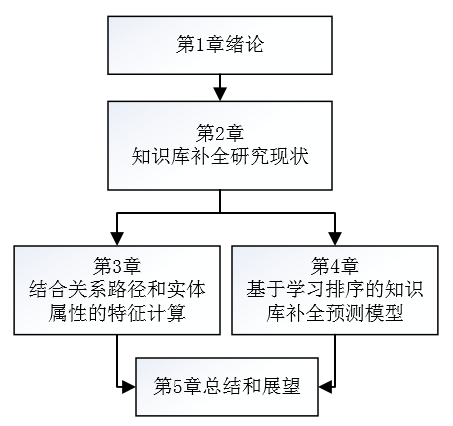
\includegraphics [width=0.63\textwidth]{intro.PNG}
\caption{论文组织结构图}
\label{kbcintro}
\end{center}
\end{figure}
\textbf{第2章} 介绍当前知识库技术的研究现状。主要包括知识库构建、知识库应用和知识库补全和推理。

\textbf{第3章}介绍了基于关系路径的知识库补全算法研究框架,介绍了如何结合关系路径类型和实体属性类型进行知识库补全算法模型预测。

\textbf{第4章}介绍了如何构建学习排序的算法进行知识库补全模型预测,包括如何构建目标函数,如何进行特征优化。

\textbf{第5章}总结了本研究工作的重点和不足,提出了未来研究的一些思路和方向。
